% 2023 新高考Ⅱ卷 20：三棱锥 A-BCD（E 为 BC 中点，点 F 满足 EF→=DA→）
% 绘制依据：源 PDF 原图 + 题设坐标 D(0,0,0)、B(2,0,0)、C(0,2,0)、A(1,1,√2)、
% E(1,1,0)（BC 中点）、F(2,2,√2)。投影：画布 = x·(1,0) + y·(0.42,0.30) + z·(0,1)，
% 得 D(0,0)、B(2,0)、C(0.84,0.60)、E(1.42,0.30)、A(1.42,1.714)、F(2.84,2.014)，
% 版面即 D 左下、B 右下（DB 近水平）、C 中部偏左（被遮挡顶点）、E 中央偏下、
% A 上方中偏左、F 右上角。实线 DB、DA、AB、AF、FB；虚线 DC、CB、CA 及 AE、DE。
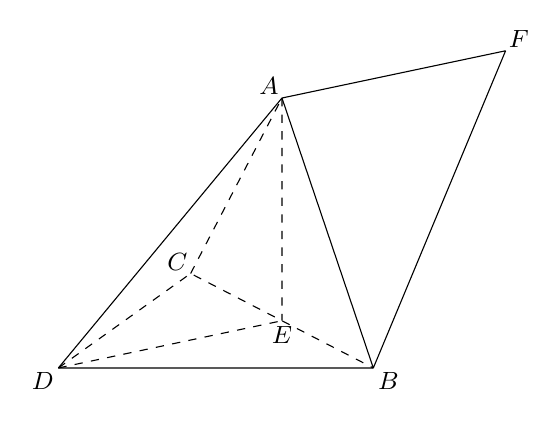
\begin{tikzpicture}[scale=2.0, font=\small]
  \coordinate (D) at (0,0);
  \coordinate (B) at (2,0);
  \coordinate (C) at (0.84,0.60);
  \coordinate (E) at (1.42,0.30);
  \coordinate (A) at (1.42,1.7142);
  \coordinate (F) at (2.84,2.0142);
  \draw (D) -- (B)  (D) -- (A)  (A) -- (B)  (A) -- (F)  (F) -- (B);
  \draw[dashed] (D) -- (C) -- (B);
  \draw[dashed] (C) -- (A);
  \draw[dashed] (A) -- (E)  (D) -- (E);
  \node[below left, inner sep=1.5pt] at (D) {$D$};
  \node[below right, inner sep=1.5pt] at (B) {$B$};
  \node[above left, inner sep=1pt] at (C) {$C$};
  \node[below, inner sep=2pt] at (E) {$E$};
  \node[above left, inner sep=1pt] at (A) {$A$};
  \node[above right, inner sep=1pt] at (F) {$F$};
\end{tikzpicture}
